\newcounter{english}
\documentclass{article}

% packages
\usepackage{amsmath, amsthm, thmtools, amsfonts, amssymb, luacode, catchfile, tikzducks, hyperref, ifthen}
\ifcsname c@kobocompile\endcsname
	\usepackage[a5paper, total={1072pt, 1448pt}, margin=10pt, includeheadfoot]{geometry} % set page margins
\else
	\usepackage[a4paper, margin=50pt, includeheadfoot]{geometry}
\fi
\usepackage[shortlabels]{enumitem}
\usepackage[skip=3pt, indent=0pt]{parskip}

% language
\usepackage[bidi=basic, layout=tabular, provide=*]{babel}
\ifcsname c@english\endcsname
	\babelprovide[main, import]{english}
\else
	\babelprovide[main, import]{hebrew}
	\babelprovide{rl}
\fi
%\babelfont{rm}{Libertinus Serif}
\babelfont{rm}[Renderer=Harfbuzz]{Libertinus Serif}
\babelfont{sf}{Libertinus Sans}
\babelfont{tt}{Libertinus Mono}

% style
\AddToHook{cmd/section/before}{\clearpage}	% Add line break before section
\linespread{1.3}
\setcounter{secnumdepth}{0}		% Remove default number tags from sections, this won't do well with theorems
\AtBeginDocument{\setlength{\belowdisplayskip}{3pt}}
\AtBeginDocument{\setlength{\abovedisplayskip}{3pt}}
\graphicspath{ {../images/} }

% operators
\DeclareMathOperator\cis{cis}
\DeclareMathOperator\Sp{Sp}
\DeclareMathOperator\tr{tr}
\DeclareMathOperator\im{Im}
\DeclareMathOperator\re{Re}
\DeclareMathOperator\diag{diag}
\DeclareMathOperator*\lowlim{\underline{lim}}
\DeclareMathOperator*\uplim{\overline{lim}}
\DeclareMathOperator\rng{rng}
\DeclareMathOperator\Sym{Sym}
\DeclareMathOperator\Arg{Arg}
\DeclareMathOperator\Log{Log}
\DeclareMathOperator\dom{dom}
\DeclareMathOperator\supp{Supp}
\DeclareMathOperator\var{Var}
\DeclareMathOperator\cov{Cov}

% commands
%\renewcommand\qedsymbol{\textbf{מש''ל}}
%\renewcommand\qedsymbol{\fbox{\emoji{lizard}}}
\newcommand{\Aa}[0]{\mathcal{A}}
\newcommand{\Bb}[0]{\mathcal{B}}
\newcommand{\CC}[0]{\mathbb{C}}
\newcommand{\Cc}[0]{\mathcal{C}}
\newcommand{\EE}[0]{\mathbb{E}}
\newcommand{\FF}[0]{\mathbb{F}}
\newcommand{\Ff}[0]{\mathcal{F}}
\newcommand{\Ii}[0]{\mathcal{I}}
\newcommand{\Gg}[0]{\mathcal{G}}
\newcommand{\Ll}[0]{\mathcal{L}}
\newcommand{\Mm}[0]{\mathcal{M}}
\newcommand{\NN}[0]{\mathbb{N}}
\newcommand{\Nn}[0]{\mathcal{N}}
\newcommand{\PP}[0]{\mathbb{P}}
\newcommand{\Pp}[0]{\mathcal{P}}
\newcommand{\QQ}[0]{\mathbb{Q}}
\newcommand{\RR}[0]{\mathbb{R}}
\newcommand{\Rr}[0]{\mathcal{R}}
\newcommand{\Ss}[0]{\mathcal{S}}
\newcommand{\TT}[0]{\mathbb{T}}
\newcommand{\Uu}[0]{\mathcal{U}}
\newcommand{\Vv}[0]{\mathcal{V}}
\newcommand{\Ww}[0]{\mathcal{W}}
\newcommand{\ZZ}[0]{\mathbb{Z}}
\newcommand{\acts}[0]{\circlearrowright}
\newcommand{\explain}[2] {
	\begin{flalign*}
		 && \text{#2} && \text{#1}
	\end{flalign*}
}
\newcommand{\maketitleprint}[0]{ \begin{center}
	%\begin{tikzpicture}[scale=3]
	%	\duck[graduate=gray!20!black, tassel=red!70!black]
	%\end{tikzpicture}	
	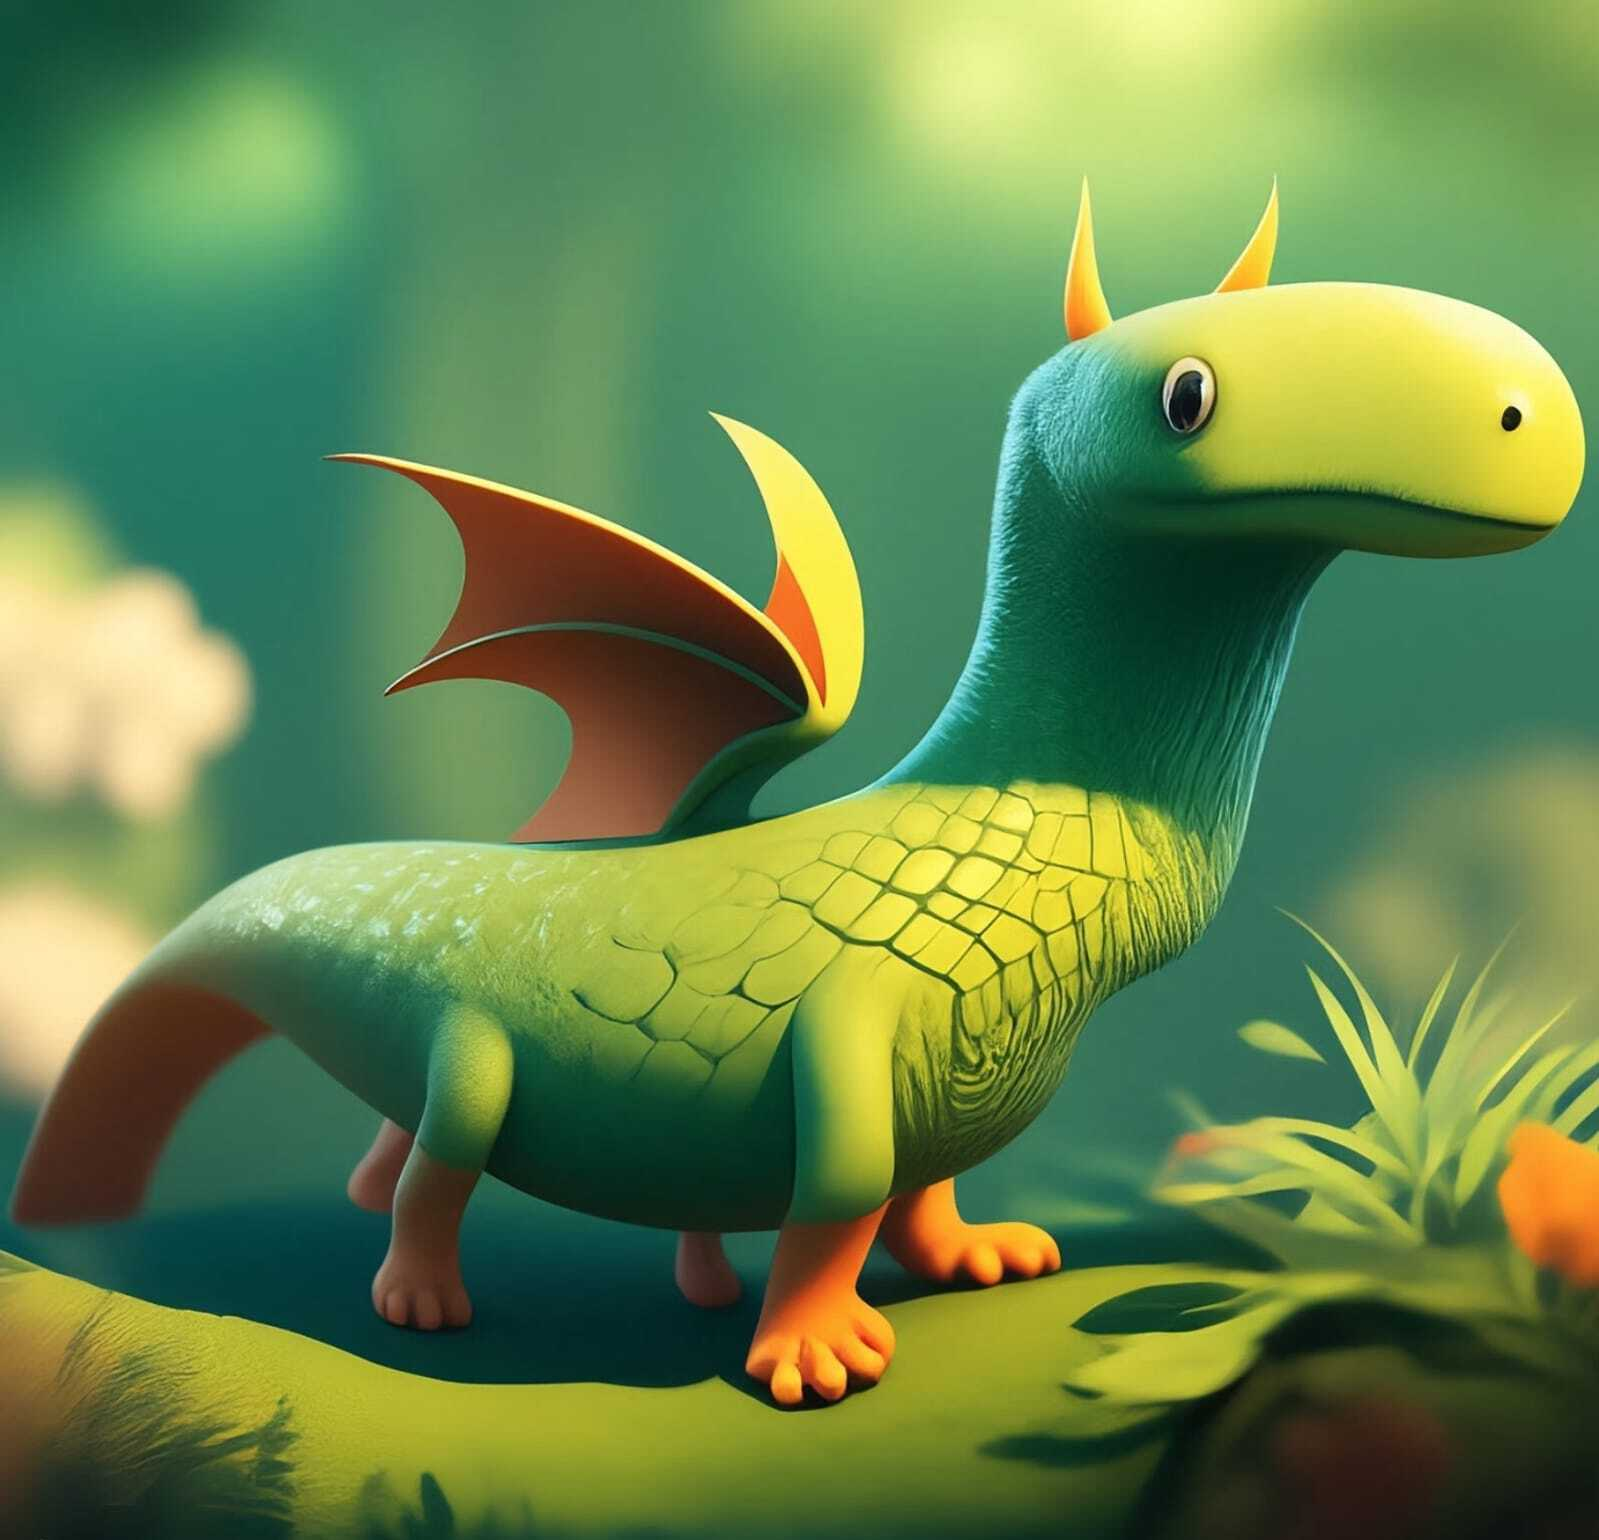
\includegraphics[width=6cm]{cover}
\end{center}
}

% theorem commands
\newtheoremstyle{c_remark}
	{}	% Space above
	{}	% Space below
	{}% Body font
	{}	% Indent amount
	{\bfseries}	% Theorem head font
	{}	% Punctuation after theorem head
	{.5em}	% Space after theorem head
	{\thmname{#1}\thmnumber{ #2}\thmnote{ \normalfont{\text{(#3)}}}}	% head content
\newtheoremstyle{c_definition}
	{3pt}	% Space above
	{3pt}	% Space below
	{}% Body font
	{}	% Indent amount
	{\bfseries}	% Theorem head font
	{}	% Punctuation after theorem head
	{.5em}	% Space after theorem head
	{\thmname{#1}\thmnumber{ #2}\thmnote{ \normalfont{\text{(#3)}}}}	% head content
\newtheoremstyle{c_plain}
	{3pt}	% Space above
	{3pt}	% Space below
	{\itshape}% Body font
	{}	% Indent amount
	{\bfseries}	% Theorem head font
	{}	% Punctuation after theorem head
	{.5em}	% Space after theorem head
	{\thmname{#1}\thmnumber{ #2}\thmnote{ \text{(#3)}}}	% head content

\ifcsname c@english\endcsname
	\theoremstyle{plain}
	\newtheorem{theorem}{Theorem}[section]
	\newtheorem{lemma}[theorem]{Lemma}
	\newtheorem{proposition}[theorem]{Proposition}
	\newtheorem*{proposition*}{Proposition}
	%\newtheorem{corollary}[theorem]{אין חלופה עברית}

	\theoremstyle{definition}
	\newtheorem{definition}[theorem]{Definition}
	\newtheorem*{definition*}{Definition}
	\newtheorem{example}{Example}[section]
	\newtheorem{exercise}{Exercise}[section]

	\theoremstyle{remark}
	\newtheorem*{remark}{Remark}
	\newtheorem*{solution}{Solution}
	\newtheorem{conclusion}[theorem]{Conclusion}
	\newtheorem{notation}[theorem]{Notation}
\else
	\theoremstyle{c_plain}
	\newtheorem{theorem}{משפט}[section]
	\newtheorem{lemma}[theorem]{למה}
	\newtheorem{proposition}[theorem]{טענה}
	\newtheorem*{proposition*}{טענה}
	%\newtheorem{corollary}[theorem]{אין חלופה עברית}

	\theoremstyle{c_definition}
	\newtheorem{definition}[theorem]{הגדרה}
	\newtheorem*{definition*}{הגדרה}
	\newtheorem{example}{דוגמה}[section]
	\newtheorem{exercise}{תרגיל}[section]

	\theoremstyle{c_remark}
	\newtheorem*{remark}{הערה}
	\newtheorem*{solution}{פתרון}
	\newtheorem{conclusion}[theorem]{מסקנה}
	\newtheorem{notation}[theorem]{סימון}
\fi

% Questions related commands
\newcounter{question}
\setcounter{question}{1}
\newcounter{sub_question}
\setcounter{sub_question}{1}

\ifcsname c@english\endcsname
	\newcommand{\question}[1][0]{
		\ifthenelse{#1 = 0}{}{\setcounter{question}{#1}}
		\section{Question \arabic{question}}
		\addtocounter{question}{1}
		\setcounter{sub_question}{1}
	}

	\newcommand{\subquestion}[1][0]{
		\ifthenelse{#1 = 0}{}{\setcounter{sub_question}{#1}}
		\subsection{Part \alph{sub_question}}
		\addtocounter{sub_question}{1}
	}
\else
	\newcommand{\question}[1][0]{
		\ifthenelse{#1 = 0}{}{\setcounter{question}{#1}}
		\section{שאלה \arabic{question}}
		\addtocounter{question}{1}
		\setcounter{sub_question}{1}
	}

	\newcommand{\subquestion}[1][0]{
		\ifthenelse{#1 = 0}{}{\setcounter{sub_question}{#1}}
		\subsection{סעיף \localecounter{letters.gershayim}{sub_question}}
		\addtocounter{sub_question}{1}
	}
\fi

% import lua and start of document
\directlua{common = require ('../common')}

\GetEnv{AUTHOR}

% headers
\author{\AUTHOR}
\date\today

\title{Exercise 2 Answer Sheet --- Logic Theory (2), 80424}

\begin{document}
\maketitle
\maketitleprint{}

\question{}
Let $F$ be a field and let $L_{F \operatorname{VS}}$ be the language of vector spaces over $F$,
$L_{F \operatorname{VS}} = \{0, +\} \cup \{ \lambda_a \mid a \in F \}$, such that $\lambda_a$ resolved to scalar multiplication.
We assume that $\Vv \subseteq \Uu$ are both infinite dimensional vector spaces over $F$, and will prove that $\Vv \prec \Uu$.
\begin{proof}
	Let us assume that $\psi(x_0, \dots, x_{n - 1})$ is a wff, as well $\varphi(x_0, \dots, x_n) = \exists x_n \psi(x_0, \dots, x_{n - 1})$.
	Let $a_0, \dots, a_{n - 1} \in V$, we will show that if $\Uu \models \varphi(a_0, \dots, a_{n - 1})$ then there is $a_n \in V$ such that $\Uu \models \psi(a_0, \dots, a_n)$.
	By the assumption that $\Uu \models \varphi(a_0, \dots, a_{n - 1})$ we assume that there is $b \in U$ such that $\Uu \models \psi(a_0, \dots, a_{n - 1}, b)$.
	If $b \in V$, then the criteria is fulfilled, then let us assume that $b \notin V$.
	Let $B_V$ be a basis for $\Vv$, it is clear that $b$ is linear-independent from $B_V$, otherwise it would follow that $b \in V$.
	We choose some $c \in V$ such that $c \in V \setminus \Sp\{ a_0, \dots, a_{n - 1} \}$, there must be one by $\Vv$'s infinite dimension.
	We construct two bases for $\Uu$, $B_U^1 \supset B_V \cup \{ b \}$, and the other one would be $B_U^2 \supset B_V \cup \{ c \}$.
	Let $M : \Uu \to \Uu$ be an automorphism such that $M(a_i) = a_i$ for all $i < n$, and let $M(b) = c$.

	We claim that $\Uu \models \psi(M(a_0), \dots, M(a_{n - 1}), M(b))$, as an automorphism is preserving any relation and function defined over its respective vector-space.
	then $c \in M$, thus being a witness to out initial claim that there is $c \in \Vv$ such that $\Uu \models \psi(a_0, \dots, a_{n - 1}, c)$.
	Tarski-Vaught tests requirements are all met, it follows that $\Vv \prec \Uu$.
\end{proof}

\question{}
\subquestion{}
We will show that if $\Mm \subseteq \Nn \subseteq \Kk$ and $\Mm \prec \Kk, \Nn \prec \Kk$, then $\Mm \prec \Nn$.
\begin{proof}
	Let $\varphi(x_0, \dots, x_{n - 1})$ be some wff, and $a_0, \dots, a_{n - 1} \in M$ then,
	\[
		\Mm \models \varphi(a_0, \dots, a_{n - 1}) \iff \Kk \models \varphi(a_0, \dots, a_{n - 1}) \iff \varphi(a_0, \dots, a_{n - 1})
	\]
	as $M \subseteq N$, hence $a_0, \dots, a_{n - 1} \in N$.
	By the definition of sub-elementary embedding, $\Mm \prec \Nn$.
\end{proof}

\subquestion{}
We will show that $\Mm = (\NN, <) \prec (\NN, <) + (\ZZ, <) = \Nn$, where addition of order models is defined as the disjoint union of the universes and the order is the lexicographic order.
\begin{proof}
	By the EF-games we showed that $\Mm \equiv \Nn$.
	We intend to use Tarski-Vaught test, it followed that we assume that $\psi(x_0, \dots, x_n)$ is a wff over $L$,
	and let $\varphi(x_0, \dots, x_{n - 1}) = \exists x_n \psi(x_0, \dots, x_n)$.
	We assume that $a_0, \dots, a_{n - 1} \in \NN$ such that $\Nn \models \varphi(a_0, \dots, a_{n - 1})$.
	We will prove that there is $a \in \Mm$ such that $\Nn \models \psi(a_0, \dots, a_{n - 1}, a)$.
	From $\Mm \equiv \Nn$ it derives that if $\phi = \exists x_0 \dots \exists x_{n - 1} \varphi(x_0, \dots, x_{n - 1})$ then $\Mm \models \phi \iff \Nn \models \phi$.
	But we assumed that $\Nn \models \varphi(a_0, \dots, a_{n - 1})$, it follows that $\Nn \models \phi$, then $\Mm \models \phi$ as well.
	Let $b_0, \dots, b_n \in \NN$ such that $\Mm \models \psi(b_0, \dots, b_n)$, the witnesses to $\Mm \models \phi$.
	It is sufficient to show that $b_i \mapsto a_i$ is an embedding of $\Mm$ into $\Mm$.
	We can assume that there is such mapping, as otherwise, it would follow that $\Mm \not\models \phi$.
	$\Mm \models \psi(a_0, \dots, a_{n - 1}, b)$ for $b$ such that the embeddings value at $b_n$, therefore $b \in N$ and $\Nn \models \psi(a_0, \dots, a_{n - 1}, b)$.
	Then by Tarski-Vaught test we deduce $\Mm \prec \Nn$.
\end{proof}

\subquestion{}
We will find an example for three models $\Mm \subseteq \Nn \subseteq \Kk$ such that $\Mm \prec \Nn, \Mm \prec \Kk$ but $\Nn \not\prec \Kk$.
\begin{solution}
	We define, $\Mm = (\NN, <), \Kk = (\NN, <) + (\ZZ, <)$ and $\Nn = (\NN, <) + (2\ZZ, <)$.
	It is inferred directly by definition that $\Mm \subseteq \Nn \subseteq \Kk$ and by the last part, $\Mm \prec \Kk$.
	We also note that $\exists x (\langle 2, 1\rangle < x < \langle 4, 1 \rangle)$ is a wff that holds in $\Nn$ but not in $\Kk$, implies that $\Nn \not\prec \Kk$.
	Lastly, by the same proof of part b, it derives that $\Mm \prec \Nn$.
\end{solution}

\question{}
\subquestion{}
We assume that $\langle f_r \mid r \in \RR \rangle$ are functions $f_r : \NN \to \NN$ such that if $r \ne q$, then there is a $k \in \NN$, such $f_r(n) \ne f_q(n)$ for all $n \ge k$.
Let $\Mm = (\NN, <, \langle f_r \mid r \in \RR \rangle)$ be structure in the language $\{ f_r \mid r \in \RR \}$.
We will show that if $\Nn \succ \Mm$ and $\Nn \ne \Mm$ then $|N| \ge |\RR|$.
\begin{proof}
	Let $\varphi_{r, q}(k) = \forall n \ge k, f_r(n) \ne f_q(n)$.
	For each $r, q \in \RR$, $\Mm \models \varphi_{r, q}(k)$ for some $k \in \NN$.
	From $\Mm \prec \Nn$ it follows that $\Nn \models \varphi_{r, q}(k)$ for $k \in \NN$ as well, for every $r, q \in \RR$.
	By the elementary embedding and the formula $\psi(x, y) = \forall z \ne x, y,\ \lnot (x < z < y)$ we can deduce that elements of $\Nn$ are not bounded by elements of $\Mm$.
	$\Nn \ne \Mm$, then there is $\alpha \in N \setminus M$, and by the last statement it derives that $n < \alpha$ for every $n \in \NN$.
	For every $r \in \RR$, $f_r(\alpha) \in N$, then by $\alpha$'s relation to the naturals we deduce that for every $r, q \in \RR$, $\Nn \models f_r(\alpha) \ne f_q(\alpha)$.
	Finally, $\{ f_r(\alpha) \mid r \in \RR \} \subseteq N$, implying that $|N| \ge |\RR|$.
\end{proof}

\subquestion{}
We will show that such a sequence of function exists.
\begin{proof}
	We define the ultrafilter $D \subseteq \Pp(\NN)$ by $X \in D \iff \exists n \in \NN, X = [n]$, that is $D$ is the collection of all finite beginnings of the natural numbers.
	We then define $\Mm = \NN^\NN / D$, in this model every elements representative is a function $\NN \to \NN$ such that it fulfills the requirement of the last part.
	Lastly, we use choice to map each such function to unique real number.
\end{proof}

\subquestion{}
We will conclude that downwards Löwenheim-Skolem theorem does not hold without the restriction of $|L|$ in the cardinality inequality, $|N| \le |L| + |A| + \aleph_0$.
\begin{proof}
	If we were to take $\Nn = (\omega_1, <, \langle f_r \mid r \in \RR \rangle)$, a model like in the first part, and the set $A = \omega + 1$, then the model $\Mm$ derived from the theorem satisfies,
	\[
		\omega_1 = |N| \le |A| + \aleph_0 = \omega
	\]
	in contradiction to $\omega_1 > \omega$.
\end{proof}

\question{}
Let us assume that $G$ is a simple group.
We will show that if $H \prec G$ then $H$ is simple.
\begin{proof}
	$H$ is a group, as the formulas to represent existence of neutral element, as well the closure to operator and existence of inverted element are all first-order.
	If a group is simple by the first isomorphism theorem for groups every $f : G \to G$ which is not trivial is bijective, meaning it is an automorphism, but we know that we can represent automorphisms by conjugation.
	It follows that for every $g, g' \in G$, exists $l \in G$ such that $l g l^{-1} = g'$, or equivalently, $\psi = \forall g, g', \exists l,\ l g l^{-1} = g'$.
	By the elementary embedding $H \models \psi$ as well, but then by $\psi$ there are not normal subgroups to $H$, as if there would be one, it would consist of $H$ and be trivial.
	We conclude that $H$ is simple.
\end{proof}

\end{document}
